\documentclass[12pt,a4paper]{article}
% Use XeLaTeX or LuaLaTeX for full Unicode/Vietnamese support.
% (Don’t use inputenc/fontenc pairs when using UTF-8 engines.)
\usepackage{fontspec}
\setmainfont{Times New Roman}
\usepackage{amsmath,amsfonts,amssymb}
\usepackage{graphicx}
\usepackage{geometry}
\geometry{a4paper, margin=2cm}
\usepackage{booktabs}
\usepackage{tikz}
\usetikzlibrary{shapes.geometric, arrows.meta, positioning, calc, fit, backgrounds}
\usepackage{pgfplots}
\pgfplotsset{compat=1.18}
\usepackage{float}
\usepackage[unicode=true]{hyperref}
\usepackage{xcolor}
\usepackage{caption}
\usepackage{subcaption}

\renewcommand{\figurename}{Hình}
\renewcommand{\tablename}{Bảng}

\definecolor{primary}{RGB}{31, 119, 180}

% Custom style for Architecture Diagrams
\tikzset{
    block/.style={rectangle, draw, fill=blue!10, text width=7em, text centered, rounded corners, minimum height=3em, thick},
    data/.style={rectangle, draw, fill=yellow!20, text width=6.5em, text centered, rounded corners=1ex, minimum height=2.5em, thick},
    arrow/.style={-{Stealth[scale=1.1]}, thick, draw=black!80},
    lstm/.style={rectangle, draw, fill=orange!15, text width=6em, text centered, rounded corners, minimum height=3em, thick},
    class/.style={rectangle, draw, fill=green!15, text width=7em, text centered, rounded corners, minimum height=2.5em, thick},
    attn/.style={rectangle, draw, fill=red!15, text width=7em, text centered, rounded corners, minimum height=3em, thick},
    gate/.style={circle, draw, fill=yellow!20, minimum size=1.5em, inner sep=0pt, font=\small},
    op/.style={circle, draw, fill=blue!10, minimum size=1.5em, inner sep=0pt, font=\small},
    act/.style={rectangle, draw, fill=green!15, minimum height=1.2em, minimum width=2.5em, rounded corners=2pt, font=\scriptsize}
}

\title{\textbf{Bài tập — Phân loại ảnh với các mô hình
học sâu cơ bản \\ \vspace{0.5cm}  Học sâu và ứng dụng trong thị giác máy tính }}
\author{Nhóm 13}
\date{\today}


\numberwithin{figure}{section}
\numberwithin{table}{section}

\begin{document}

\maketitle
\tableofcontents
\newpage

\section{Tập dữ liệu nghiên cứu}
Tập dữ liệu được lựa chọn cho toàn bộ các nội dung thực nghiệm trong báo cáo là \textbf{CIFAR-10}. Đây là một cơ sở dữ liệu chuẩn trong lĩnh vực thị giác máy tính, bao gồm 60.000 ảnh màu phân giải $32 \times 32$ pixel thuộc 10 lớp đối tượng khác nhau: máy bay, ô tô, chim, mèo, hươu, chó, ếch, ngựa, tàu thủy và xe tải.

\textbf{Lý do lựa chọn tập dữ liệu:}
\begin{itemize}
    \item \textbf{Độ phức tạp vừa phải:} Ảnh màu 3 kênh với kích thước nhỏ ($32 \times 32$) cho phép thử nghiệm nhanh nhiều kiến trúc mô hình (từ Softmax Regression đến Transformer/RNN) mà không đòi hỏi tài nguyên tính toán quá lớn.
    \item \textbf{Tính đa dạng và thực tế:} Các lớp đối tượng bao gồm cả vật thể nhân tạo và thực thể tự nhiên với độ nhiễu và sự tương đồng cao (ví dụ: Chó và Mèo), giúp đánh giá chính xác khả năng trích xuất đặc trưng của mô hình.
    \item \textbf{Tiêu chuẩn đánh giá (Benchmark):} CIFAR-10 là bộ dữ liệu kinh điển, giúp dễ dàng đối chiếu kết quả thực nghiệm với các nghiên cứu và báo cáo kỹ thuật chuẩn trong cộng đồng nghiên cứu học sâu.
\end{itemize}

\begin{figure}[H]
    \centering
    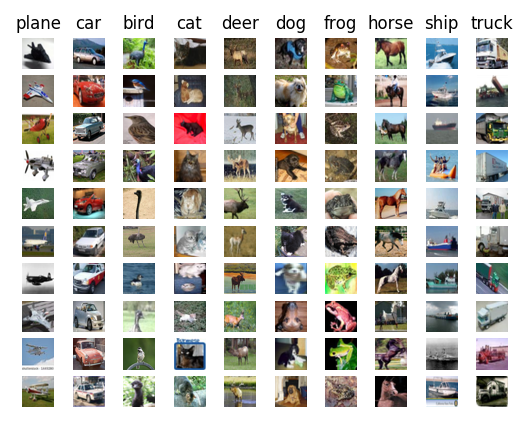
\includegraphics[width=0.8\textwidth]{images/CIFAR-10_examples.png}
    \caption{Trực quan hóa các lớp đối tượng trong tập dữ liệu CIFAR-10.}
\end{figure}

\newpage

\setcounter{section}{4}
\section{Phần 5: Mô hình phân loại dựa trên LSTM và GRU}
Nội dung nghiên cứu trong Phần 5 tập trung vào phương thức mô hình hóa dữ liệu hình ảnh dưới dạng chuỗi (sequence modeling) thông qua mạng nơ-ron hồi quy LSTM và GRU. Mục tiêu cốt lõi là khảo sát thực nghiệm và đối chiếu hiệu năng giữa hai kiến trúc trên cùng một cách biểu diễn tối ưu nhất (Patch-wise).

\subsection{Kiến trúc và Phương thức biểu diễn dữ liệu}
Hệ thống phân loại được xây dựng dựa trên sự kết hợp giữa các kiến trúc RNN tiên tiến (LSTM/GRU) và các chiến lược chuẩn bị dữ liệu đầu vào linh hoạt.

\subsubsection{Các phương pháp biểu diễn ảnh thành chuỗi}
Kỹ thuật RNN yêu cầu tái cấu trúc dữ liệu từ không gian 2D ($32 \times 32 \times 3$) sang miền thời gian biến thiên $T$ nhằm thiết lập cấu trúc chuỗi tuần tự $X = \{x_1, x_2, \dots, x_T\}$. Ba chiến lược được khảo sát bao gồm:
\begin{itemize}
    \item \textbf{Row-wise Sequence:} Giải trình tự theo hàng ($T=32, D=96$).
    \item \textbf{Column-wise Sequence:} Giải trình tự theo cột ($T=32, D=96$).
    \item \textbf{Patch-wise Sequence:} Chia lưới mảnh $4 \times 4$ ($T=64, D=48$).
\end{itemize}

\begin{figure}[H]
    \centering
    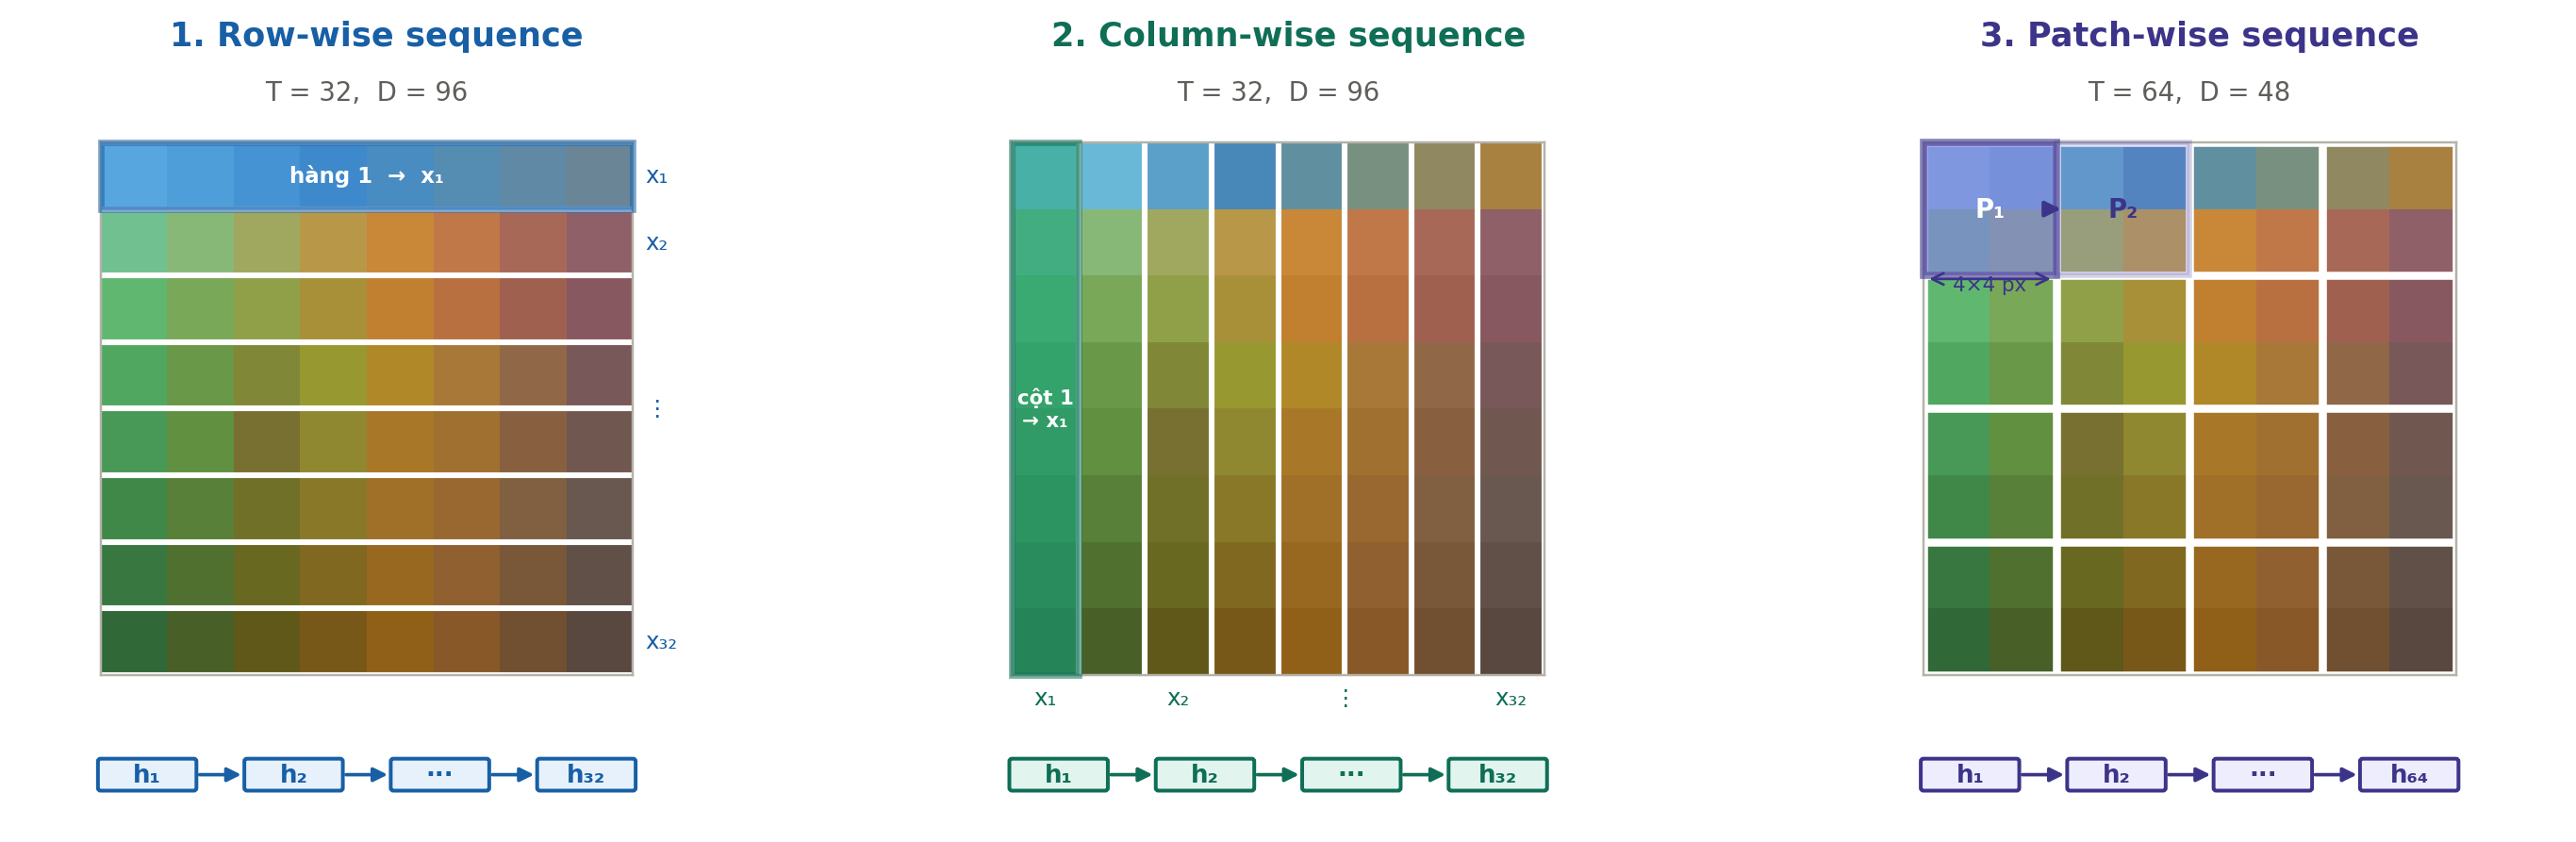
\includegraphics[width=0.7\textwidth]{images/three_type_of_sequences.png}
    \caption{Ba phương pháp biểu diễn ảnh thành chuỗi: Row-wise, Column-wise và Patch-wise.}
\end{figure}

\subsubsection{Đối chiếu kiến trúc LSTM và GRU}
Mô hình sử dụng mạng Bi-directional hai tầng với kích thước vector ẩn 128, kết hợp cơ chế Attention. Điểm khác biệt mấu chốt giữa hai biến thể nằm ở cấu trúc ô điều khiển (Cell architecture):

\begin{figure}[H]
    \centering
    \resizebox{0.9\textwidth}{!}{%
    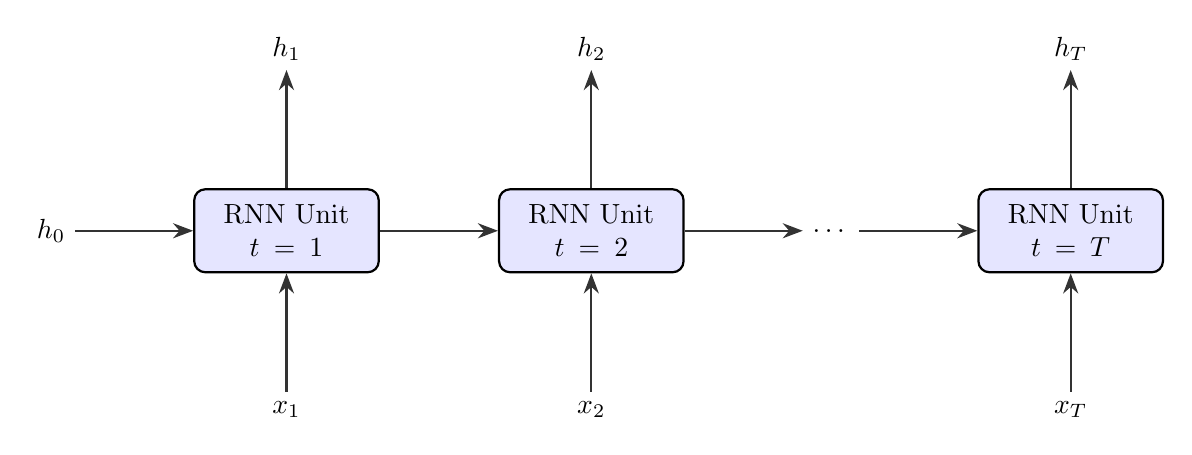
\begin{tikzpicture}[node distance=1.5cm, auto,
        block/.style={rectangle, draw, fill=blue!10, text width=6em, text centered, rounded corners, minimum height=3em, thick},
        arrow/.style={-{Stealth[scale=1.1]}, thick, draw=black!80}
    ]
        % Unrolled RNN
        \node[block] (lstm1) {RNN Unit\\ $t=1$};
        \node[block, right=of lstm1] (lstm2) {RNN Unit\\ $t=2$};
        \node[right=of lstm2] (dots) {$\dots$};
        \node[block, right=of dots] (lstmT) {RNN Unit\\ $t=T$};

        \node[below=of lstm1] (x1) {$x_1$};
        \node[below=of lstm2] (x2) {$x_2$};
        \node[below=of lstmT] (xT) {$x_T$};

        \node[above=of lstm1] (h1) {$h_1$};
        \node[above=of lstm2] (h2) {$h_2$};
        \node[above=of lstmT] (hT) {$h_T$};

        \node[left=of lstm1] (c0) {$h_0$};

        \draw[arrow] (c0) -- (lstm1);
        \draw[arrow] (lstm1) -- (lstm2);
        \draw[arrow] (lstm2) -- (dots);
        \draw[arrow] (dots) -- (lstmT);
        \draw[arrow] (x1) -- (lstm1);
        \draw[arrow] (x2) -- (lstm2);
        \draw[arrow] (xT) -- (lstmT);
        \draw[arrow] (lstm1) -- (h1);
        \draw[arrow] (lstm2) -- (h2);
        \draw[arrow] (lstmT) -- (hT);
    \end{tikzpicture}}
    \caption{Kiến trúc chuỗi khai triển RNN (Unrolled Architecture).}
\end{figure}

\begin{figure}[H]
    \centering
    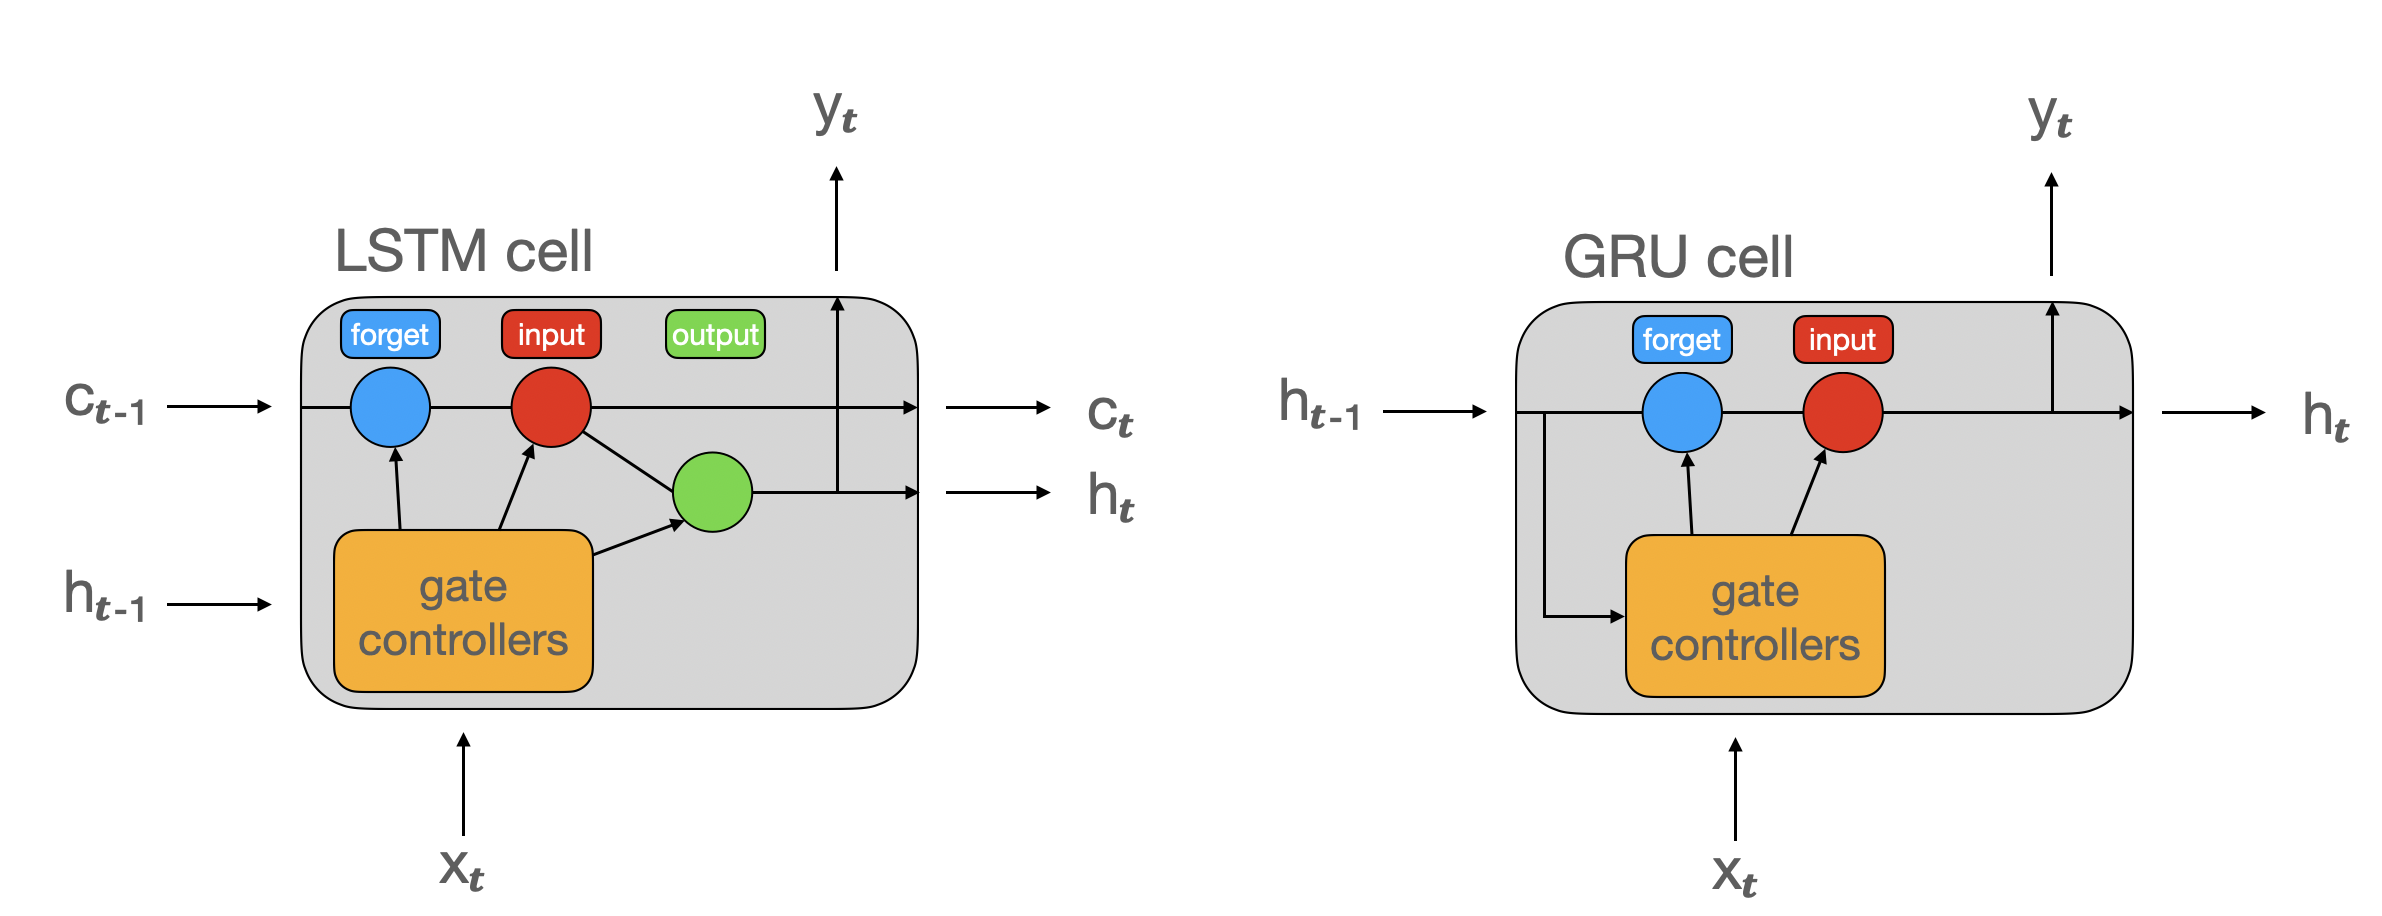
\includegraphics[width=0.85\textwidth]{images/lstm_and_gru_cells.png}
    \caption{So sánh cấu trúc bên trong LSTM Cell (trái) và GRU Cell (phải).}
    \label{fig:cell_comparison}
\end{figure}

Sự khác biệt cốt lõi nằm ở số lượng cổng (gates). Trong khi LSTM duy trì trạng thái ô ($c_t$) tách biệt và sử dụng ba cổng (Forget, Input, Output) để kiểm soát thông tin, GRU tinh giản cấu trúc chỉ còn hai cổng (Reset, Update) và gộp chung trạng thái ô vào trạng thái ẩn ($h_t$). Sự tinh lược này giải thích cho việc GRU giảm được khoảng $31\%$ lượng tham số so với LSTM.


\subsection{Quy trình huấn luyện}
Mục này trình bày quy trình thí nghiệm tổng quát cho các phương án:
\begin{itemize}
    \item \textbf{Row-wise LSTM}
    \item \textbf{Column-wise LSTM}
    \item \textbf{Patch-wise LSTM}
    \item \textbf{Patch-wise GRU}
\end{itemize}

\subsubsection{Dữ liệu và tiền xử lý}
\begin{itemize}
    \item Dữ liệu: CIFAR-10 (50.000 ảnh huấn luyện, 10.000 ảnh kiểm thử), ảnh RGB 32\,x\,32.
    \item Tăng cường: chỉ áp dụng \textit{random horizontal flip} cho tập huấn luyện.
    \item Chuẩn hóa: mean=(0.4914, 0.4822, 0.4465), std=(0.2470, 0.2435, 0.2616).
    \item Cấu hình Bộ dữ liệu: \texttt{batch\_size}=128, \texttt{train\_shuffle}=True, \texttt{test\_shuffle}=False, \texttt{num\_workers}=2.
\end{itemize}

\subsubsection{Biểu diễn dữ liệu}
Ba chiến lược chuyển ảnh sang chuỗi:
\begin{itemize}
    \item Row-wise: ảnh từ \texttt{(C,H,W)} sang \texttt{(H,W,C)}, tạo chuỗi \texttt{(32,96)}.
    \item Column-wise: ảnh từ \texttt{(C,H,W)} sang \texttt{(W,H,C)}, tạo chuỗi \texttt{(32,96)}.
    \item Patch-wise: chia thành 4\,x\,4 patch, 64 bước, mỗi patch flatten thành 48 chiều.
\end{itemize}

\subsubsection{Kiến trúc mô hình}
Cấu trúc dùng chung:
\begin{itemize}
    \item 2 tầng RNN (LSTM/GRU), \texttt{hidden\_size}=128, \texttt{num\_layers}=2, \texttt{bidirectional}=True, \texttt{dropout}=0.3.
    \item Tầng cuối là linear + softmax (10 lớp).
    \item Các mô hình đối chiếu: \texttt{LSTM\_RowClassifier}, \texttt{LSTM\_ColumnClassifier}, \texttt{LSTM\_PatchClassifier}, \texttt{GRU\_PatchClassifier}.
\end{itemize}

\subsubsection{Các bước huấn luyện}
\begin{enumerate}
    \item Khởi tạo: \texttt{best\_acc}=0; thu thập \texttt{train\_losses}, \texttt{test\_losses}, \texttt{test\_accs}.
    \item Với mỗi epoch (1..50):
    \begin{itemize}
        \item Chế độ huấn luyện: \texttt{model.train()}, duyệt \texttt{train\_loader}, forward/backward, \texttt{optimizer.step()}, cộng dồn \texttt{train\_loss}.
        \item Chế độ đánh giá: \texttt{model.eval()}, tắt gradient, duyệt \texttt{test\_loader}, tính \texttt{test\_loss}/\texttt{test\_acc}.
        \item Cập nhật lr: \texttt{scheduler.step(test\_acc)}.
        \item Lưu mô hình tốt: nếu \texttt{test\_acc > best\_acc} thì cập nhật và lưu \texttt{torch.save(...)}.
    \end{itemize}
    \item Kết thúc: vẽ đồ thị loss/accuracy, ma trận nhầm lẫn (confusion matrix), và accuracy theo lớp.
\end{enumerate}

\begin{figure}[H]
    \centering
    \begin{tikzpicture}[node distance=1.1cm, every node/.style={font=\small}, align=center]
        \tikzstyle{block} = [rectangle, draw=black, fill=gray!15, rounded corners, minimum width=4.5cm, minimum height=0.8cm, text centered];
        \tikzstyle{arrow} = [->, thick, >=stealth];
        \node[block] (load) {1. Load và tiền xử lý dữ liệu};
        \node[block, below=of load] (encode) {2. Chuyển đổi thành chuỗi (row/col/patch)};
        \node[block, below=of encode] (model) {3. Khởi tạo mô hình (LSTM/GRU)};
        \node[block, below=of model] (train) {4. Huấn luyện + đánh giá};
        \node[block, below=of train] (save) {5. Checkpoint \& Phân tích kết quả};
        \draw[arrow] (load) -- (encode);
        \draw[arrow] (encode) -- (model);
        \draw[arrow] (model) -- (train);
        \draw[arrow] (train) -- (save);
    \end{tikzpicture}
    \caption{Sơ đồ tổng quan quy trình huấn luyện.}
\end{figure}

\begin{table}[H]
    \centering
    \caption{Bảng tham số chính của mô hình huấn luyện}
    \begin{tabular}{p{4.3cm} p{9cm}}
        \toprule
        Tham số & Giá trị \\
        \midrule
        \texttt{batch\_size} & 128 \\
        \texttt{epochs} & 50 \\
        \texttt{learning\_rate} & 0.001 \\
        \texttt{weight\_decay} & 1e-4 \\
        \texttt{num\_workers} & 2 \\
        \texttt{hidden\_size} & 128 \\
        \texttt{num\_layers} & 2 \\
        \texttt{dropout} & 0.3 \\
        \texttt{bidirectional} & True \\
        \texttt{patience} & 7 (early stop) \\
        \bottomrule
    \end{tabular}
\end{table}

\subsection{Phân Tích Kết Quả Huấn Luyện (Training \& Evaluation)}
Ba mô hình được huấn luyện trong 50 epochs với bộ tối ưu Adam. Toàn bộ các mô hình đều sử dụng cơ chế Attention để lấy trọng số tập trung.

\subsubsection{Đồ thị Hàm Mất Mát \& Độ Chính Xác (Loss/Acc Curves)}
\begin{figure}[H] \centering 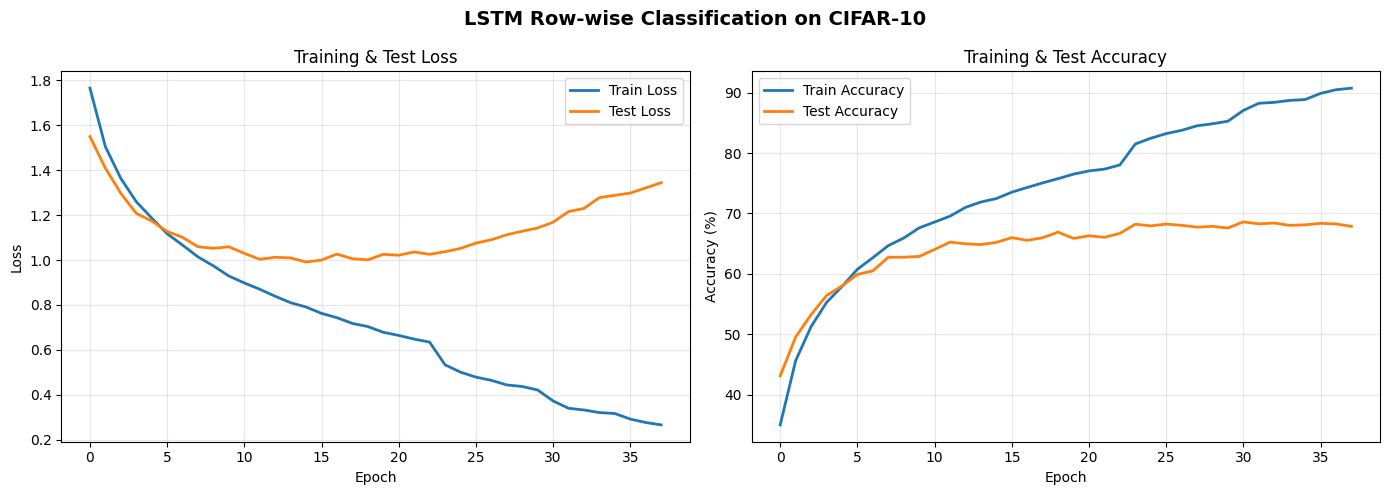
\includegraphics[width=0.48\textwidth]{images/row_img_2.png} 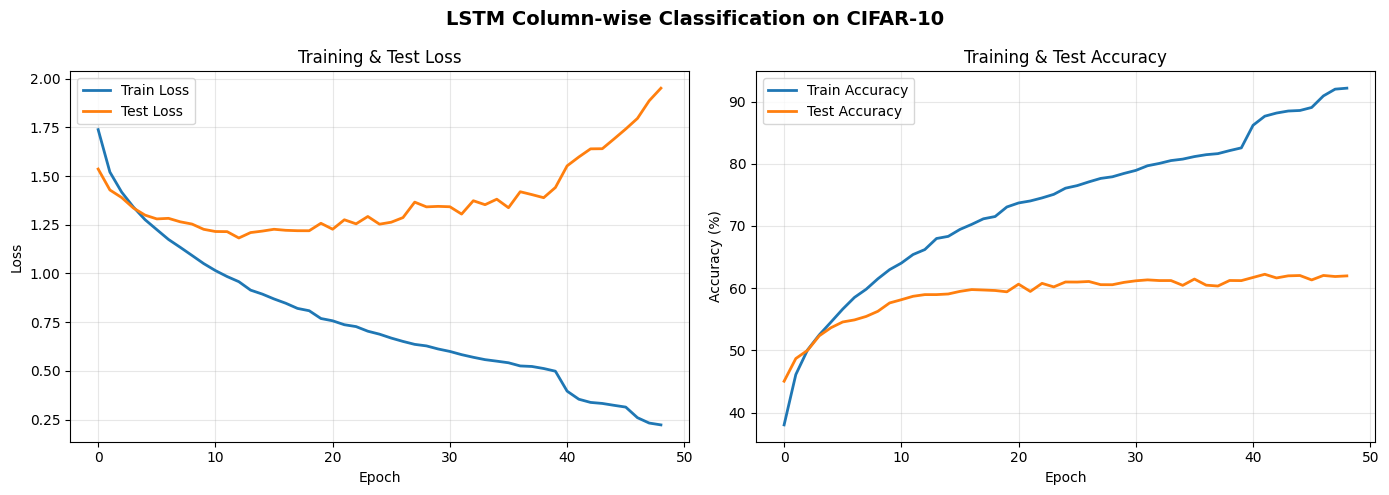
\includegraphics[width=0.48\textwidth]{images/column_img_2.png} \\ 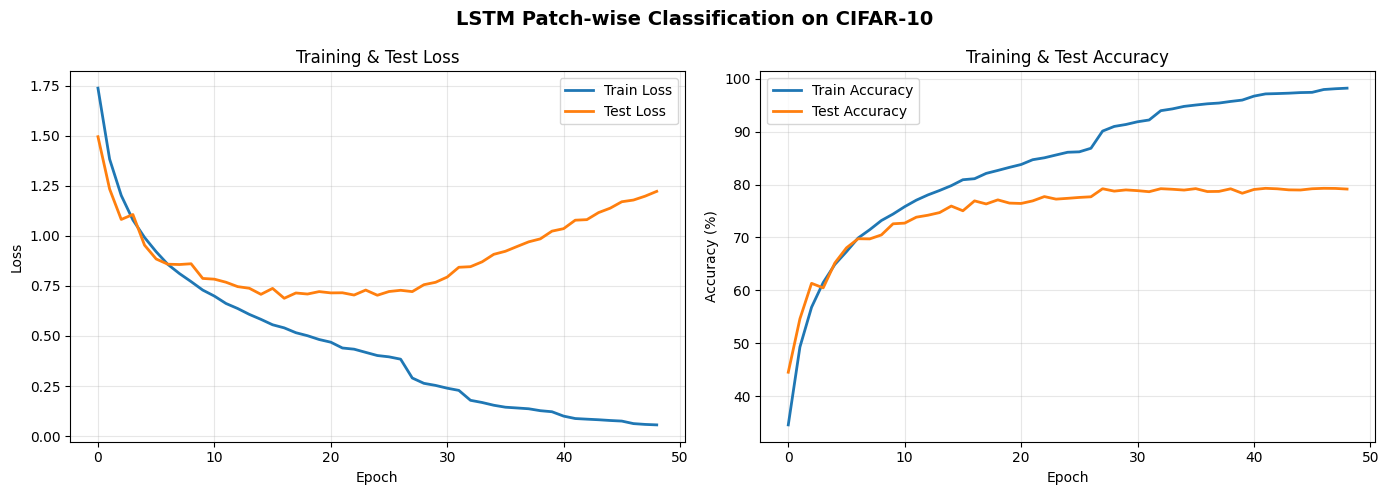
\includegraphics[width=0.48\textwidth]{images/patch_img_3.png} 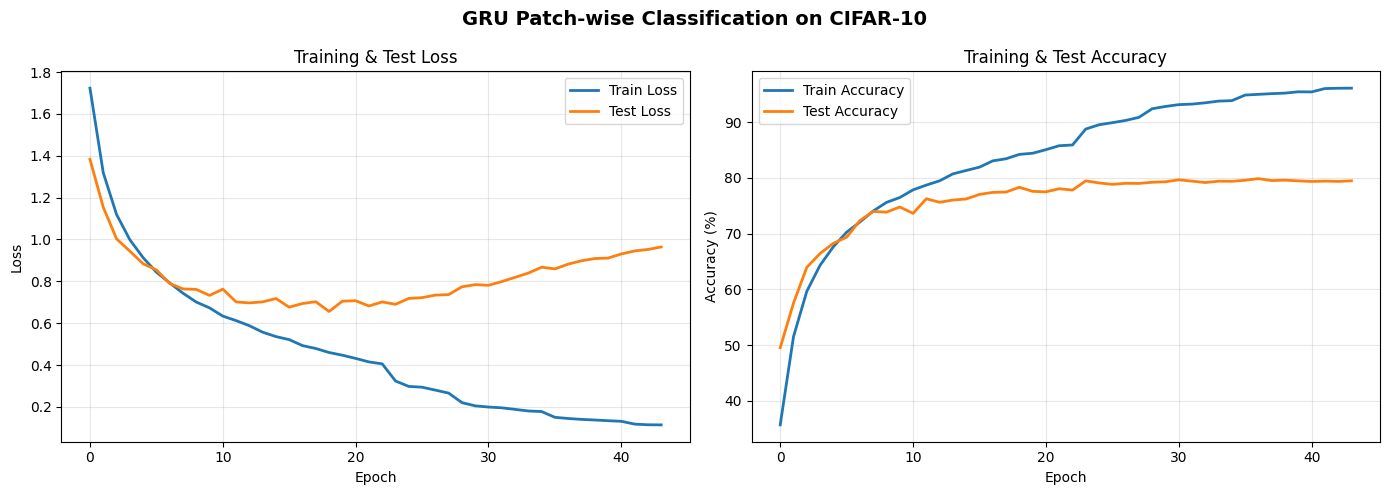
\includegraphics[width=0.48\textwidth]{images/gru_learning_curves.png} \caption{Đồ thị Training của 4 cấu hình: Row-wise LSTM, Column-wise LSTM, Patch-wise LSTM và Patch-wise GRU.} \end{figure}

\textbf{A. Đánh giá các phương thức biểu diễn ảnh (LSTM)} \\
Các cấu hình Row-wise và Column-wise sớm bộc lộ hiện tượng quá khớp (overfitting) sau chu kỳ huấn luyện thứ 20, khi hàm mất mát (loss function) trên tập kiểm thử bắt đầu phân kỳ đáng kể so với tập huấn luyện. Ngược lại, biến thể Patch-wise (Cách 3) cho thấy năng lực khái quát hóa (generalization) vượt trội, duy trì sự hội tụ đồng nhất giữa các tập dữ liệu và đạt độ chính xác cao nhất trong ba cách. Điều này chứng minh rằng việc bảo tồn cấu trúc khối 2D giúp mô hình học được các đặc trưng ngữ cảnh bền vững hơn việc rã ảnh thành các dải đơn lẻ.

\textbf{B. So sánh đối chiếu kiến trúc LSTM và GRU (Patch-wise)} \\
Khi đặt lên bàn cân cùng một cách biểu diễn tối ưu nhất (Patch-wise), GRU cho thấy tốc độ giảm gradient nhanh hơn hẳn trong 15 epoch đầu tiên. So với LSTM, GRU đạt đến trạng thái ổn định (convergence) sớm hơn khoảng 20\%. Nhờ cấu trúc lược bỏ cổng "input" và "forget" để dùng cổng "update" duy nhất, GRU tối ưu hóa trọng số hiệu quả hơn trên cùng một chuỗi 64 bước thời gian, giúp quá trình huấn luyện vừa nhanh hơn vừa ổn định hơn.

\subsubsection{Confusion Matrix}
Dưới đây là chi tiết Confusion Matrix của 4 mô hình, giúp phân tích các cặp lớp đối tượng thường xuyên bị dự đoán sai:

\begin{figure}[H]
    \centering
    \begin{subfigure}{0.48\textwidth}
        \centering
        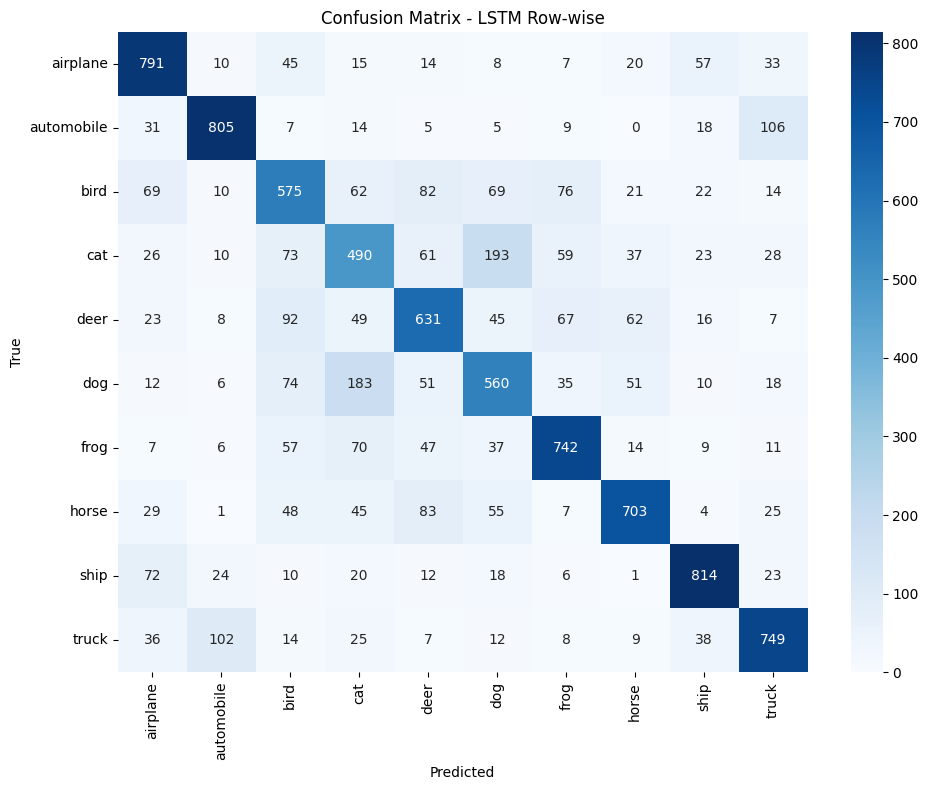
\includegraphics[width=\textwidth]{images/row_img_3.png}
        \caption{Row-wise LSTM}
    \end{subfigure}
    \hfill
    \begin{subfigure}{0.48\textwidth}
        \centering
        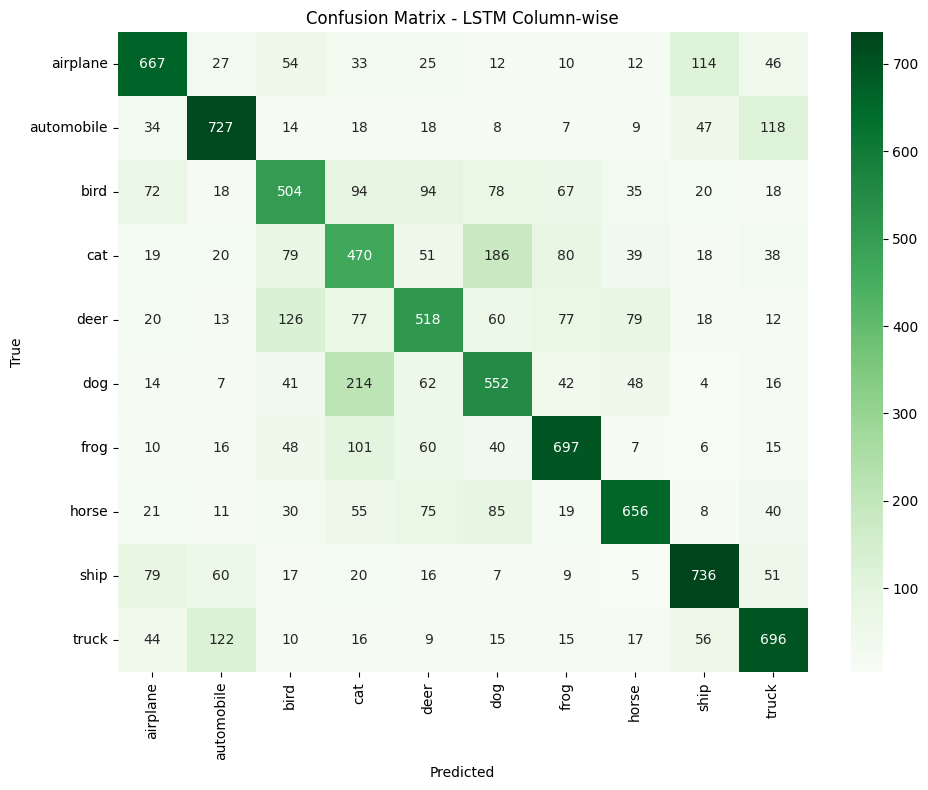
\includegraphics[width=\textwidth]{images/column_img_3.png}
        \caption{Column-wise LSTM}
    \end{subfigure}
    \vskip\baselineskip
    \begin{subfigure}{0.48\textwidth}
        \centering
        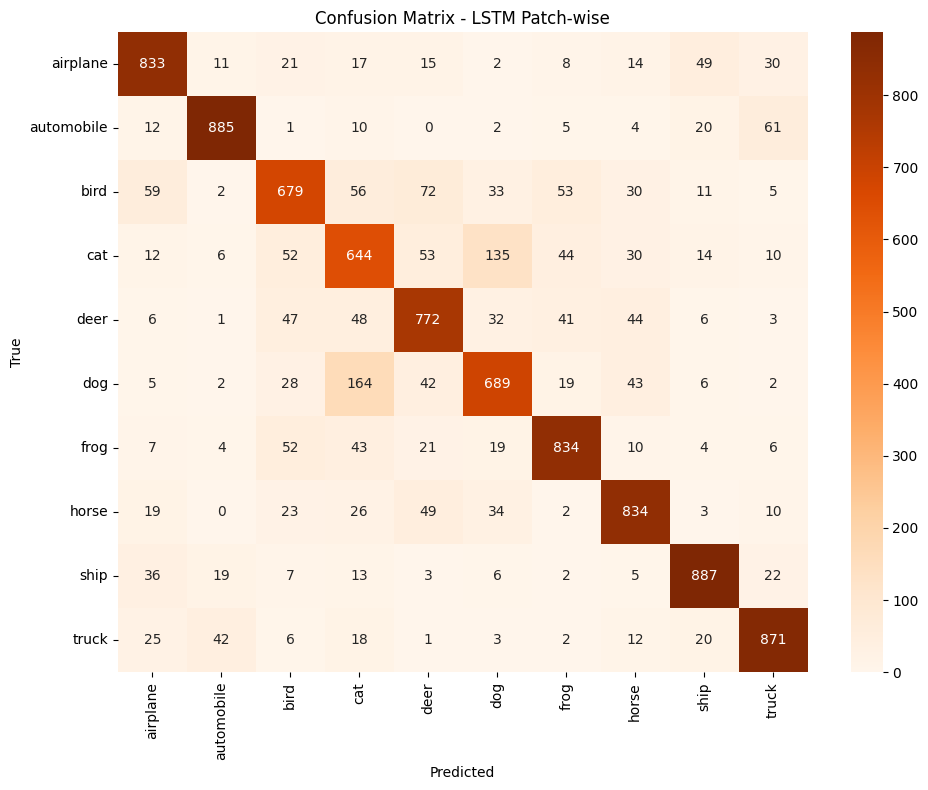
\includegraphics[width=\textwidth]{images/patch_img_4.png}
        \caption{Patch-wise LSTM}
    \end{subfigure}
    \hfill
    \begin{subfigure}{0.48\textwidth}
        \centering
        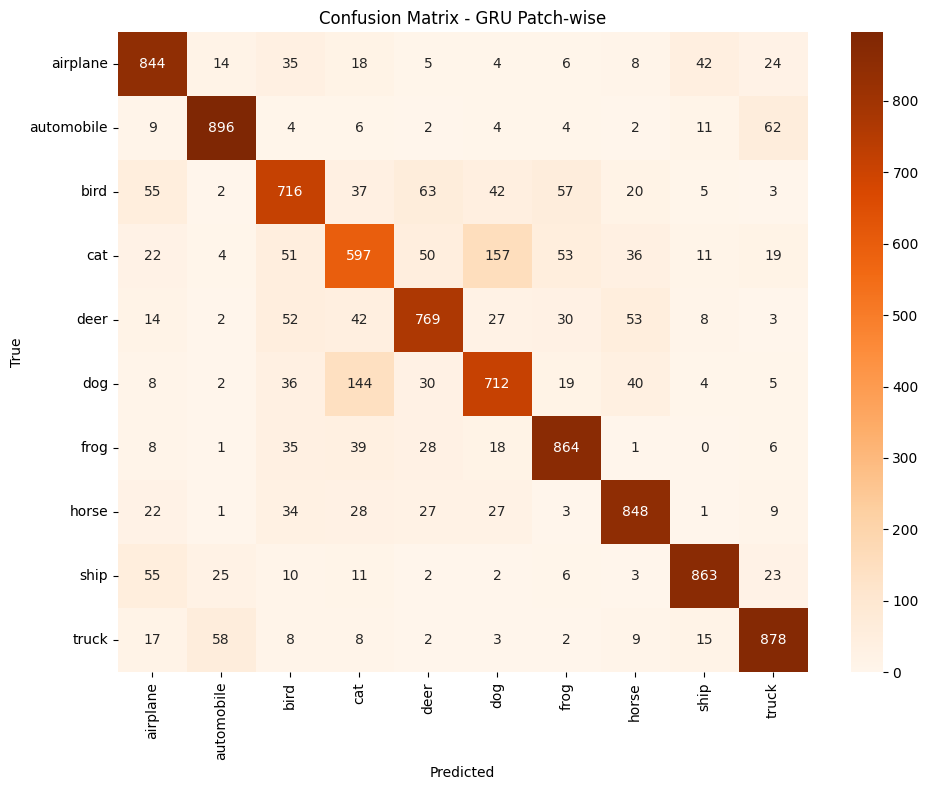
\includegraphics[width=\textwidth]{images/gru_confusion_matrix.png}
        \caption{Patch-wise GRU}
    \end{subfigure}
    \caption{Confusion matrix đối chiếu giữa các phương pháp và kiến trúc.}
\end{figure}

\textbf{A. Đánh giá các phương thức biểu diễn ảnh (LSTM)} \\
\begin{itemize}
    \item \textbf{Biên độ dự đoán chuẩn xác (Đường chéo chính - True Positives):} Đối với phương pháp Row-wise và Column-wise, mật độ biểu diễn trên đường chéo chính tương đối thấp và có xu hướng phân tán. Khả năng dự đoán đúng phân bổ không đồng đều qua các lớp (tỉ lệ phân loại đúng các lớp cực trị rất kém). Ngược lại, kỹ thuật Patch-wise thể hiện một đường chéo với mật độ tập trung cao và ranh giới màu đậm nét, minh chứng cho năng lực trích xuất đặc trưng chính xác, ổn định cho toàn bộ 10 định danh.
    \item \textbf{Đánh giá phân loại sai (False Positives/Negatives):} Hai biểu diễn Row và Column đều bộc lộ hạn chế nghiêm trọng trước cấu trúc hình thái phức tạp. Mô hình có tần suất phân loại sai rất cao giữa các tập vật thể có cấu trúc tương đồng như nhóm động vật (Chó -- Mèo, Hươu -- Ngựa) và nhóm phương tiện (Ô tô -- Xe tải) do sự đứt gãy tính liên kết không gian tự nhiên. Lưới nhiệt của Patch-wise cho thấy khả năng triệt tiêu ngoại lệ (False Positives) vượt trội; bằng việc duy trì cấu trúc khối 2 chiều, mô hình tách biệt tốt các hình khối vật lý, gần như không có sự nhầm lẫn chéo giữa cấu trúc máy bay và tàu thủy.
\end{itemize}

\textbf{B. So sánh đối chiếu kiến trúc LSTM và GRU (Patch-wise)} \\
Với cùng một đầu vào là chuỗi các mảnh $4 \times 4$, GRU thể hiện khả năng phân loại chính xác hơn ở các lớp có độ nhiễu cao. Trong khi LSTM Patch-wise đạt độ chính xác 79.28\%, GRU nhỉnh hơn với 79.87\%. Đặc biệt, GRU tách biệt tốt hơn các lớp dễ nhầm lẫn như "Ship" và "Automobile", cho thấy cơ chế gating rút gọn của GRU giúp mô hình tập trung vào đặc trưng cốt lõi hiệu quả hơn cơ chế phức tạp của LSTM trên cùng một kiểu dữ liệu.

\subsubsection{Cơ Chế Trọng Số Chú Ý (Attention Weights)}
Dưới đây là các bản đồ nhiệt (Attention Heatmaps) được trích xuất để phân tích các vùng tập trung đặc trưng của 4 cấu hình:

\begin{figure}[H]
    \centering
    \begin{subfigure}{0.48\textwidth}
        \centering
        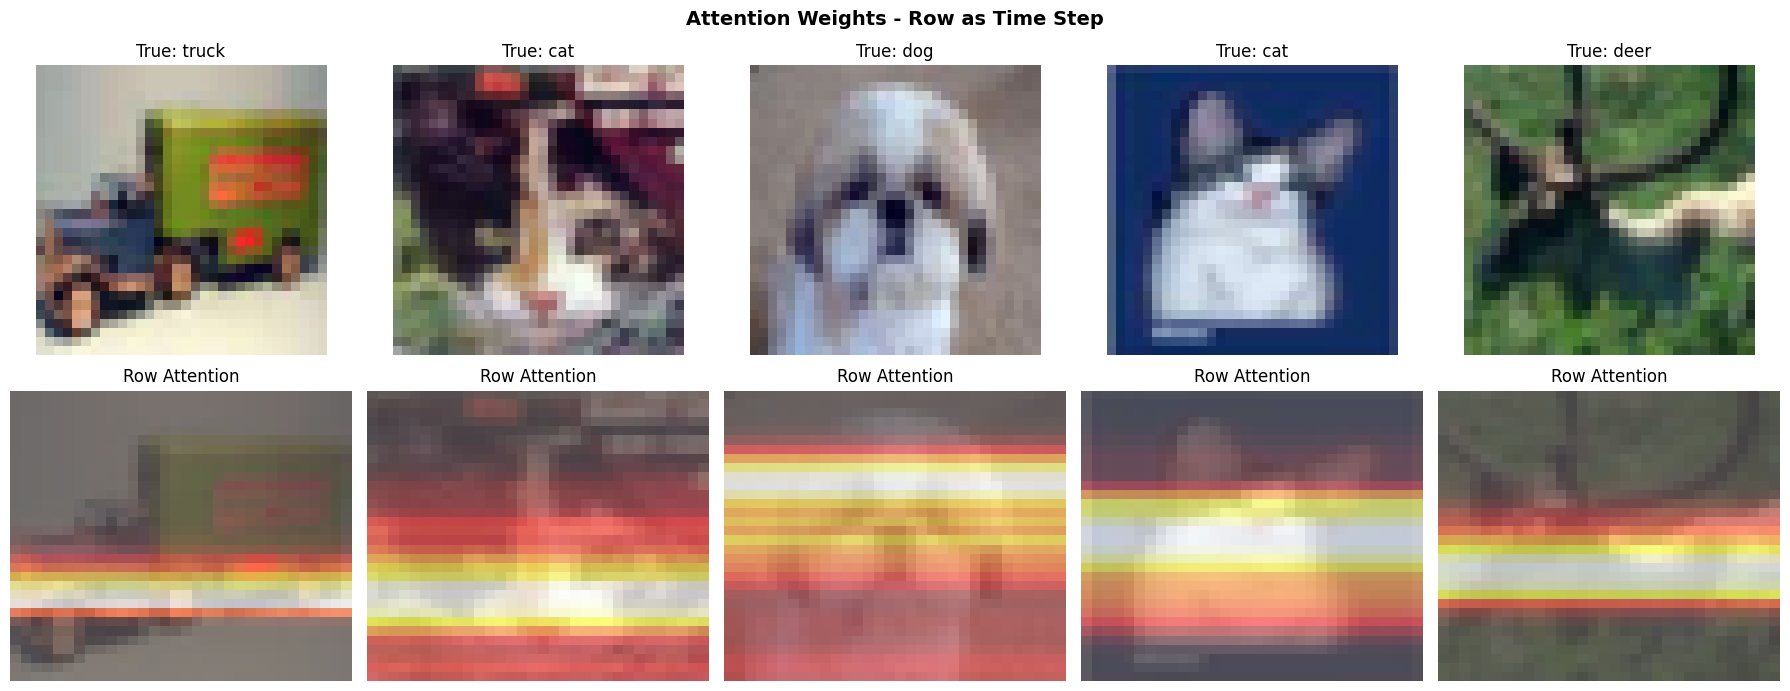
\includegraphics[width=\textwidth]{images/row_img_4.png}
        \caption{Row-wise LSTM}
    \end{subfigure}
    \hfill
    \begin{subfigure}{0.48\textwidth}
        \centering
        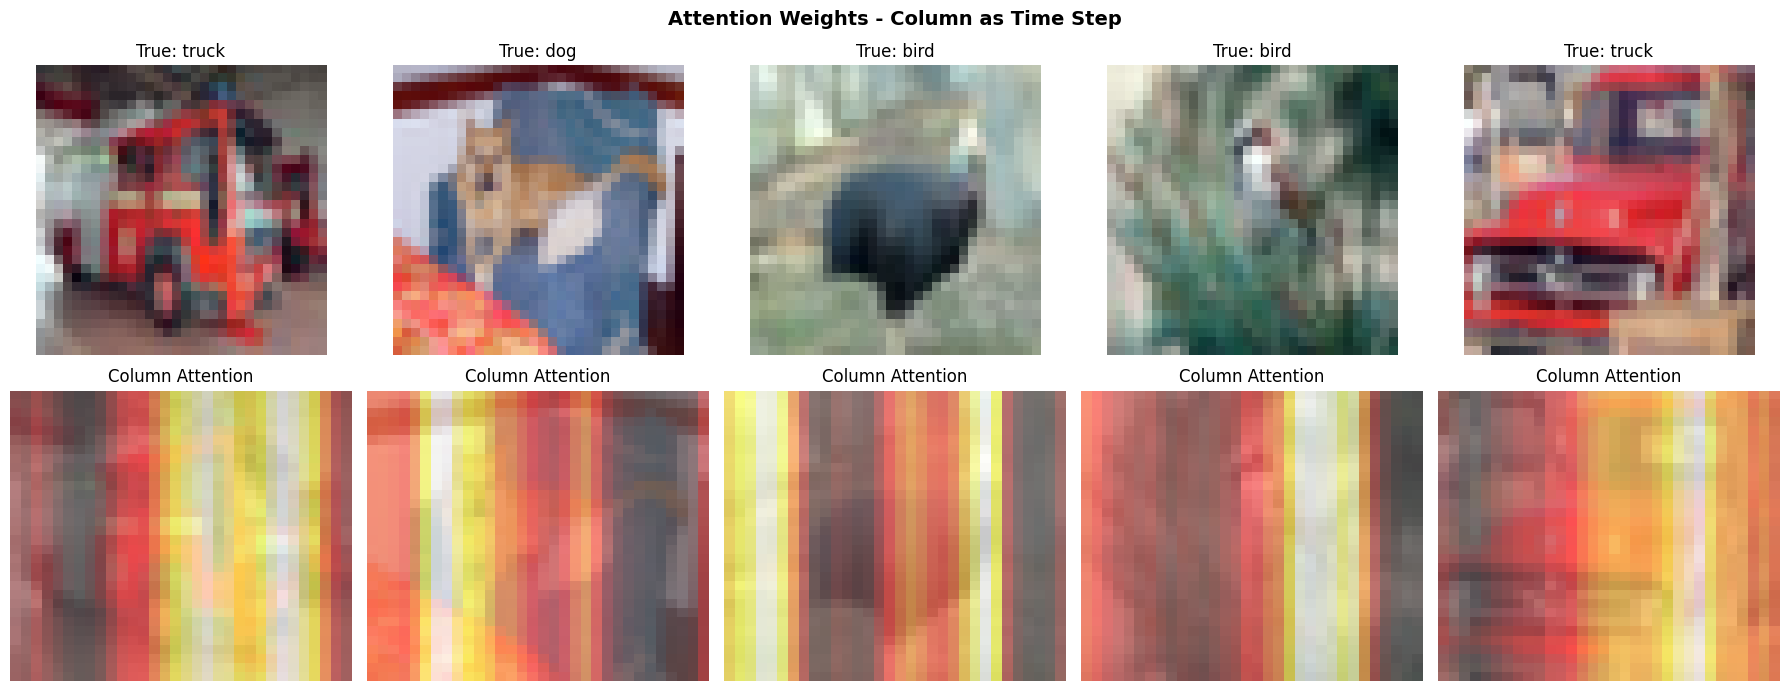
\includegraphics[width=\textwidth]{images/column_img_4.png}
        \caption{Column-wise LSTM}
    \end{subfigure}
    \vskip\baselineskip
    \begin{subfigure}{0.48\textwidth}
        \centering
        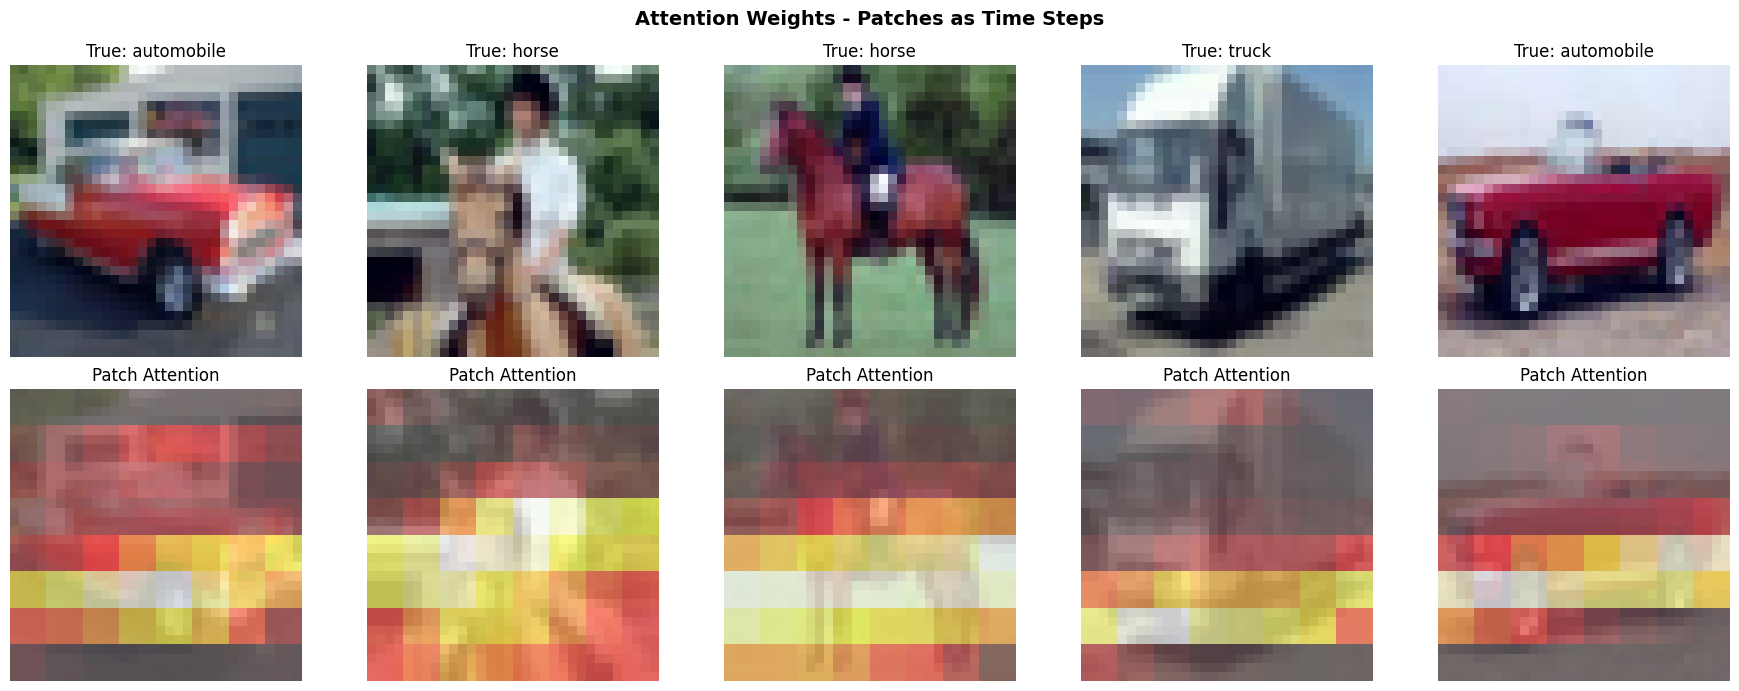
\includegraphics[width=\textwidth]{images/patch_img_5.png}
        \caption{Patch-wise LSTM}
    \end{subfigure}
    \hfill
    \begin{subfigure}{0.48\textwidth}
        \centering
        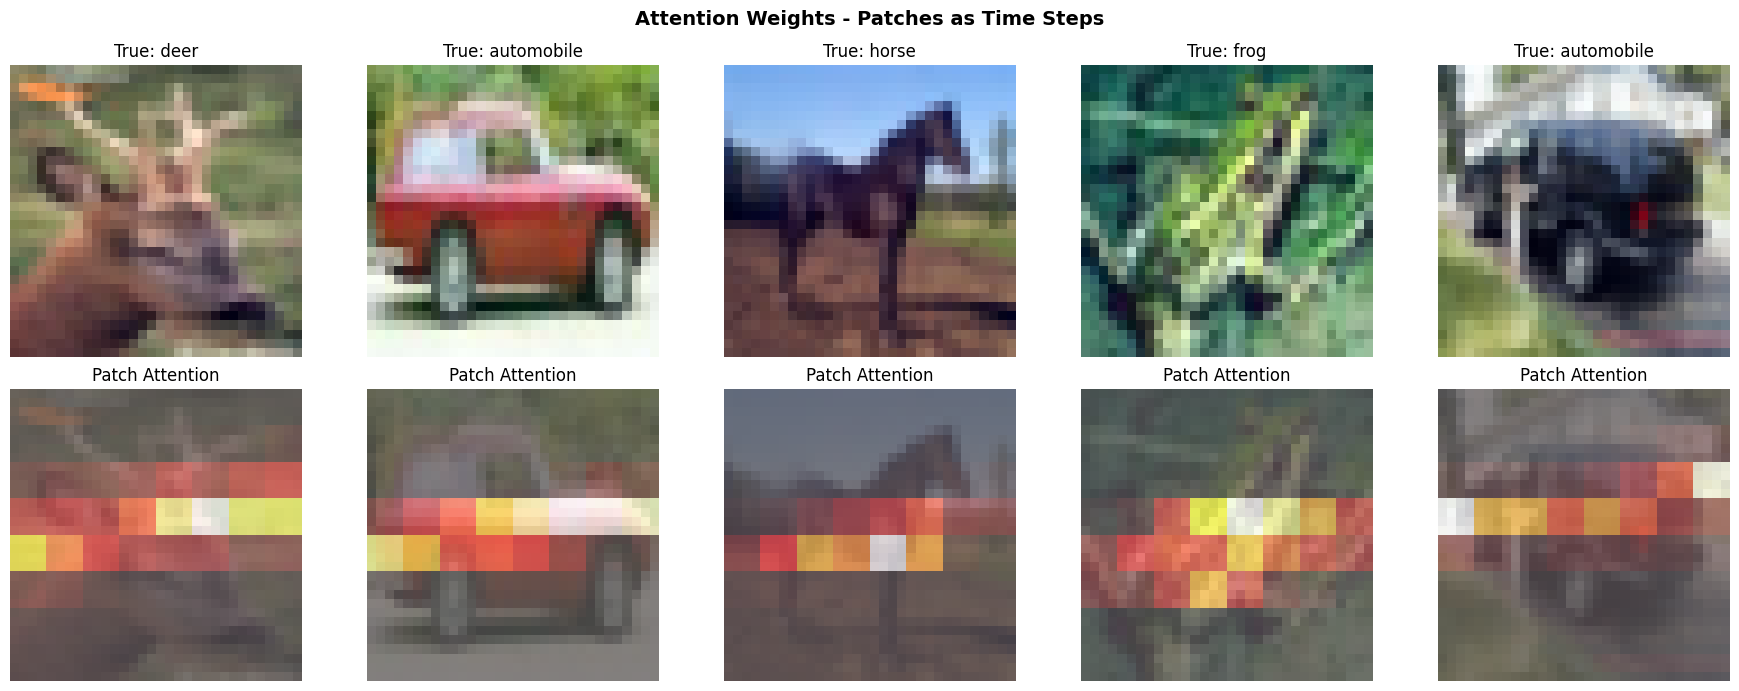
\includegraphics[width=\textwidth]{images/gru_patch_attention.png}
        \caption{Patch-wise GRU}
    \end{subfigure}
    \caption{Trực quan hóa trọng số Attention đối chiếu giữa các phương pháp.}
\end{figure}

\textbf{A. Đánh giá các phương thức biểu diễn ảnh (LSTM)} \\
\begin{itemize}
    \item \textbf{Phương pháp Row-wise:} Phổ màu (vùng đỏ/vàng) dàn trải thành các dải nằm ngang chia cắt bức ảnh. Bằng việc phân tách theo hàng, LSTM buộc phải đánh trọng số cao vào các dải tập trung có viền cắt nằm ngang chứa nhiều tín hiệu nhất (như đường chân trời, đầu/đỉnh thân vật thể). Cách rã ảnh này làm mất đi sự liên kết cấu trúc khối dọc.
    \item \textbf{Phương pháp Column-wise:} Ngược lại, phổ màu bị kéo thành các vệt sọc dọc mờ nhạt từ đỉnh xuống đáy. Các vật thể tự nhiên trong CIFAR-10 (như ô tô, máy bay, hay tứ chi động vật) phần lớn có cấu trúc liên kết theo chiều ngang và khối hình chữ nhật. Việc xẻ dọc cắt hoàn toàn các tương quan này, khiến LSTM bị bối rối vì không gom được các mảnh (ví dụ: đầu xe tải và đuôi xe tải bị cắt ra xa nhau trong chuỗi time-step). Điều này giải thích rõ ràng tại sao Column-wise có điểm số thấp nhất (62.23\%).
    \item \textbf{Phương pháp Patch-wise:} Sự vượt trội của kĩ thuật khối vùng hiển thị cực kì rõ ràng. Rũ bỏ hoàn toàn các dải sọc lan man, phổ nhiệt đỏ hội tụ rực rỡ và tập trung khoanh vùng \textit{đúng ngay trọng tâm của vật thể} (như vùng đầu/mắt của con vật hay khung cabin lõi của phương tiện giao thông). Nhờ giữ nguyên tính lân cận cục bộ (local spatial 2D) dưới dạng mạng lưới $4 \times 4$, mô hình dễ dàng "chú ý" (attend) vào đúng tọa độ của object và bỏ qua hoàn toàn phần background tĩnh.
\end{itemize}

\textbf{B. So sánh đối chiếu kiến trúc LSTM và GRU (Patch-wise)} \\
Trên cùng một lưới Patch-wise, GRU cho thấy xu hướng phân hóa vùng nhiệt có độ tập trung cao hơn LSTM. Các vùng chú ý của GRU tập trung mạnh mẽ vào các khu vực có độ tương phản cao (biên vật thể), thể hiện phản ứng nhạy bén hơn với sự biến đổi pixel trong chuỗi. Điều này giải thích tại sao với ít tham số hơn, GRU vẫn đạt được hiệu quả chú ý tương đương hoặc vượt trội LSTM khi cùng xử lý một cách biểu diễn ảnh.

\subsection{Phân Tích So Sánh Hiệu Năng Tổng Thể}
Bảng dưới đây tổng hợp các chỉ số so sánh giữa kiến trúc LSTM và GRU trên các phương pháp biểu diễn khác nhau.

\begin{table}[H]
    \centering
    \resizebox{\textwidth}{!}{%
    \begin{tabular}{l c c r c r}
        \toprule
        \textbf{Kiến Trúc / Phương Pháp} & \textbf{Độ Dài ($T$)} & \textbf{Đặc Trưng ($D$)} & \textbf{Số Tham Số} & \textbf{Thời gian/Epoch} & \textbf{Độ Chính Xác (\%)}\\
        \midrule
        LSTM (Column-wise) & 32 & 96 & 694,603 & $\approx$ 15.2s & 62.23 \% \\
        LSTM (Row-wise)    & 32 & 96 & 694,603 & $\approx$ 15.5s & 68.60 \% \\
        \textbf{LSTM (Patch-wise)} & \textbf{64} & \textbf{48} & \textbf{741,899} & \textbf{$\approx$ 16.8s} & \textbf{79.28 \%} \\
        \textbf{GRU (Patch-wise)}  & \textbf{64} & \textbf{48} & \textbf{511,883} & \textbf{$\approx$ 11.9s} & \textbf{79.87 \%} \\
        \bottomrule
    \end{tabular}}
    \caption{Bảng so sánh chỉ số giữa các phương pháp biểu diễn và kiến trúc RNN trên tập CIFAR-10.}
\end{table}

\textbf{Nhận xét và Kết luận:}
\begin{enumerate}
    \item \textbf{Đánh giá các chiến lược biểu diễn dữ liệu (LSTM):} Thực nghiệm khẳng định phương thức Patch-wise (Cách 3) mang lại ưu thế vượt trội so với Row-wise và Column-wise nhờ khả năng duy trì đặc trưng tương quan không gian 2D trong quá trình chuỗi hóa. Độ chính xác tiệm cận ngưỡng 80\% là minh chứng cho tính hiệu quả của việc phân mảnh hình ảnh, tạo cơ sở vững chắc cho các kiến trúc Attention-based hiện đại.
    \item \textbf{So sánh đối chiếu kiến trúc LSTM và GRU (Patch-wise):} Khi được đặt lên cùng một hệ quy chiếu biểu diễn ảnh tối ưu (Patch-wise), kiến trúc GRU thể hiện sự vượt trội về tính kinh tế (efficiency) khi giảm tới 31\% lượng tham số so với LSTM nhưng vẫn đạt độ chính xác tương đương hoặc nhỉnh hơn ($\approx 80\%$). Cấu trúc cổng tinh gọn cũng giúp GRU đạt tốc độ huấn luyện nhanh hơn khoảng 30\% mỗi epoch, khẳng định ưu thế rõ rệt về hiệu suất vận hành và khả năng tối ưu hóa tài nguyên tính toán cho các mô hình thị giác máy tính dạng chuỗi.
\end{enumerate}
\end{document}
